\chapter{บทนำ}
\label{chapter:introduction}

\section{ที่มาและความสำคัญ}

บริษัท ไซเจ็น เป็นบริษัทที่บริการและให้คำปริกษาและบริการโซลูชั่น SAP ในองค์กรต่างๆมากมาย และพัฒนาคิดค้นนวัตกรรมใหม่ๆ เพื่อช่วยแก้ปัญหาในองค์กร ทำให้ธุรกิจสามารถดำเนินไปได้อย่างราบรื่นมากยิ่งขึ้น เช่น การทำ SAP BUINESS ONE ช่วยทำให้เห็นภาพรวามของการทำธุรกิจได้อย่างชัดเจน,  การทำ RPA (Robotic Process Automation) โรบอทที่จะมาช่วยทำงานออฟฟิศแทนมนุษย์ และ BUDDY RECRUIT เทคโนโลยีที่ช่วยให้บริษัทหาคนเข้ามาทำงานได้ตรงตามความต้องการของบริษัทนั้นๆ

การรับสมัครงาน เป็นกระบวนการที่ทุกๆบริษัทต้องมีเพื่อที่จะรับพนักงาน ที่มีความสามารถตรงตามที่บริษัทนั้นๆต้องการ ในปัจจุบันกระบวนการรับสมัครงานของแต่ละบริษัทส่วนใหญ่ ก่อนที่จะมีการสัมภาษณ์งานเกิดขึ้น ทางบริษัทจะดูข้อมูลของผู้สมัครผ่านทางเรซูเม่ เพื่อดูประสบการณ์การทำงาน และทักษะต่างๆที่ผู้สมัครมี แต่ถ้าหากมีผู้สมัครเป็นจำนวนมาก อาจทำให้ใช้ระยะเวลาในการคัดกรองผู้สมัครงานที่มากขึ้นตามไปด้วย และผู้ที่มาสมัครนั้นอาจมีความสามารถไม่ตรงตามความต้องการของบริษัท

ในการปฏิบัติงานครั้งนี้ ผมได้เป็นในสมาชิกของทีม BUDDY RECRUIT โดยได้รับมอบหมายงานให้ทำเว็บแอพพลิเคชั่นประเมินความสามารถเบื้องต้นของผู้สมัครงาน เพื่อให้บริษัท สามารถรู้ได้เบื้องต้นว่าพนักงานที่มาสมัครมีความสามารถตรงตามความต้องการของบริษัทหรือไม่ และระบบนี้ยังมีความสามารถมากมายที่จะช่วยลดระยะเวลาในการสร้างข้อสอบเพื่อคัดกรองผู้ที่มาสมัครงานอีกด้วย เช่น การคัดลอกข้อสอบที่มีพนักงานในบริษัทได้สร้างไว้แล้วสามารถแก้ไขข้อสอบนั้นๆได้, การส่งอีเมลให้ผู้สมัครงานทำข้อสอบโดยอัติโนมัติ หรือการสุ่มข้อสอบตามระดับความยากที่พนักงานได้กำหนดไว้

\section{วัตถุประสงค์การปฏิบัติงาน}

\begin{enumerate}
  \item ศึกษาเทคโนโลยีใหม่ๆ ที่ใช้ในการทำงาน
  \item พัฒนากระบวนการคิด และการลงมือทำในสายงาน Full Stack Developer
  \item พัฒนาทักษะการทำงานภายใต้แรงกดดัน และระยะเวลาที่จำกัด
  \item พัฒนาทักษะการแก้ไขปัญหาเฉพาะหน้า
  \item ศึกษากระบวนการทำงานภายในทีม
  \item พัฒนาทักษะการสื่อสาร
  \item นำความรู้ที่ได้ ไปต่อยอดกับงานในอนาคต
\end{enumerate}

\section{ประวัติ และรายละเอียดบริษัท}

\subsection{ชื่อสถานประกอบการ}

ชื่อบริษัท(ภาษาไทย): บริษัท ไซเจ็น จำกัด

ชื่อบริษัท(ภาษาอังกฤษ): ZyGen Company Limited

\subsection{สถานที่ตั้ง}

65/60 ชั้น 6 อาคารชำนาญเพ็ญชาติบิสเนสเซ็นเตอร์ ถนนพระราม 9 เขตห้วยขวาง, กรุงเทพ -มหานคร 10310

\subsection{ลักษณะสถานประกอบการ}

บริษัท ไซเจ็น เป็นบริษัทที่บริการและให้คำปรึกษาและบริการโซลูชัน SAP ในองค์กรต่างๆมากมาย และพัฒนาคิดค้นนวัตกรรมใหม่ๆ เพื่อช่วยแก้ปัญหาในองค์กร ทำให้ธุรกิจสามารถดำเนินไปได้อย่างราบรื่นมากยิ่งขึ้น ไซเจ็น เป็นบริษัทที่มีฐานลูกค้าที่มั่นคง และยังเพิ่มฐานลูกค้าต่อไป ตัวอย่างการให้บริการของ ไซเจ็น เช่น การทำ SAP BUINESS ONE ช่วยทำให้เห็นภาพรวามของการทำธุรกิจได้อย่างชัดเจน,  การทำ RPA (Robotic Process Automation) โรบอทที่จะมาช่วยทำงานออฟฟิศแทนมนุษย์ และ BUDDY RECRUIT เทคโนโลยีที่ช่วยให้บริษัทหาคนเข้ามาทำงานได้ตรงตามความต้องการของบริษัทนั้นๆ

\begin{figure}[H]
  \centering
  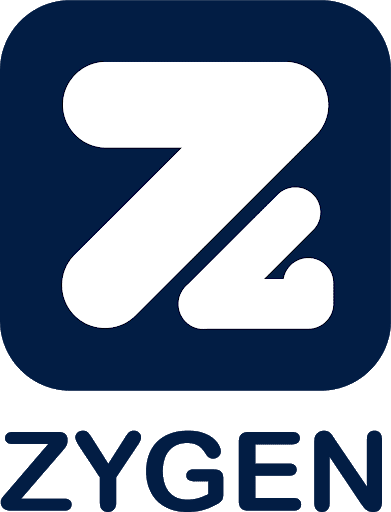
\includegraphics[width=0.4\columnwidth]{zygen-logo.png}
  \caption{ตราสัญลักษณ์ของ บริษัท ไซเจ็น}
  \label{Fig:zygen-logo}
\end{figure}

\begin{figure}[H]
  \centering
  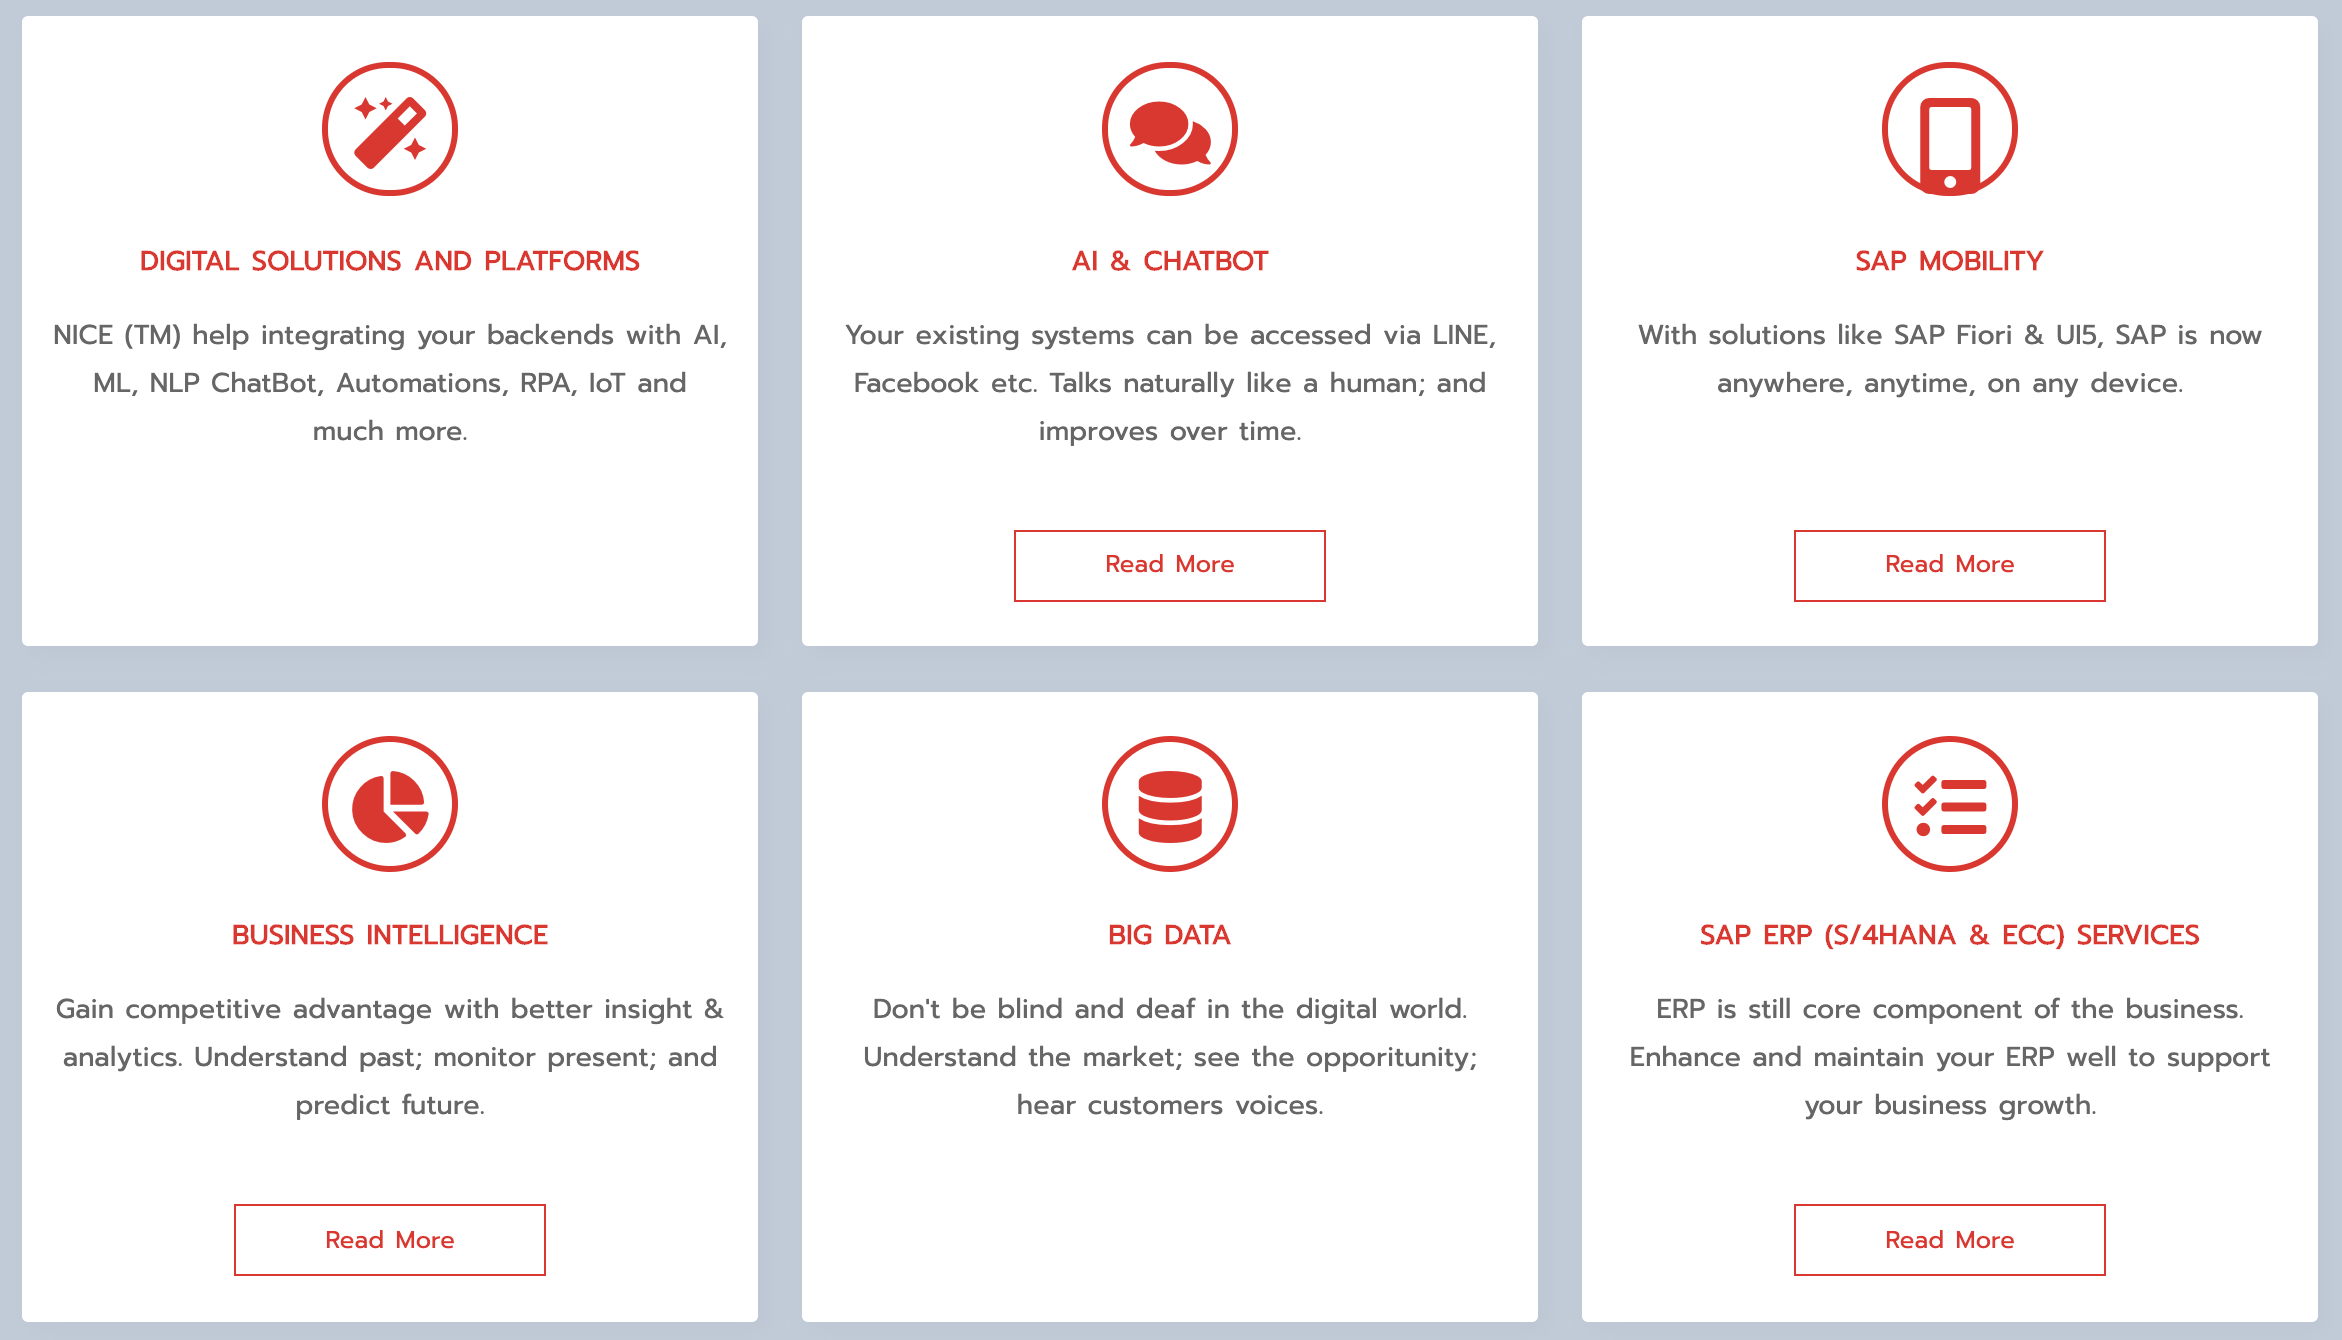
\includegraphics[width=1\columnwidth]{zygen-services.png}
  \caption{ตัวอย่างการให้บริการของ บริษัท ไซเจ็น}
  \label{Fig:zygen-services}
\end{figure}

\subsection{ตำแหน่งและลักษณะงานที่นักศึกษาได้รับมอบหมายให้รับผิดชอบ}

ตำแหน่ง: Full Stack Developer

หน้าที่: พัฒนาเว็บแอพพลิเคชั่นตามความต้องการของลูกค้า

\subsection{ชื่อและตำแหน่งของพนักงานที่ปรึกษา}

ชื่อ-นามสกุล: นายวิวัฒน์ เส็งอนันต์

ตำแหน่ง: Web Developer

แผนก: Development Team

\subsection{ระยะเวลาปฏิบัติงาน}

ช่วงเวลาปฏิบัติงาน: 1 มิถุนายน 2563 - 30 กันยายน 2563

ช่วงเวลาปฏิบัติงาน: จันทร์ - ศุกร์ เวลา 09:00 น. - 18:00 น.

รวมระยะเวลา: 4 เดือน


